\documentclass[a4paper,14pt]{article}

% Packages
\usepackage{graphicx}  % For images
\usepackage{amsmath}   % For math symbols

% Define argmin command
\DeclareMathOperator*{\argmin}{arg\,min}
\usepackage{hyperref}  % For hyperlinks
\usepackage{fancyhdr}  % For headers
\usepackage{geometry}  % For page layout
\usepackage{xcolor}   % For colors
\usepackage{listings} % For code snippets
\usepackage{float}     % For image positioning
% \usepackage[format=plain,justification=center]{caption}
\usepackage[utf8]{inputenc} % For special characters
\geometry{a4paper, margin=1in}
\usepackage{pgfplots}
\usepackage{tikz}
\pgfplotsset{compat=1.18}

% Fancy header/footer settings
\pagestyle{fancy}
% clear header and footer
\fancyhf{}
\fancyfoot[R]{\thepage} % Right-align page number in the footer


% Title information
\title{Lab Report: Text, Audio, and Image Data Manipulation}
\author{107474-Joseane Pereira \\
109050-Gabriel Costa \\
108538-Francisco Gonçalves \\
Universidade de Aveiro, DETI}
\date{\today}


\begin{document}
\begin{figure}
    \centering
    
\includegraphics[width=0.3\linewidth]{ua.pdf}
    \label{fig:enter-label}
\end{figure}
\maketitle
\newpage
\tableofcontents
\newpage

\section{Introduction}
This project implements a video codec system using both intra-frame and inter-frame compression techniques. The implementation focuses on efficient compression while maintaining video quality through predictive coding, motion estimation, and Golomb encoding.

\section{System Architecture}

\subsection{Core Components}
The system consists of four main components:
\begin{itemize}
    \item \textbf{BitStream}: Handles bit-level I/O operations for binary file manipulation
    \item \textbf{Golomb Codec}: Implements Golomb-Rice coding for entropy encoding
    \item \textbf{Audio Codec}: Audio compression using predictive and inter-channel coding
    \item \textbf{Image Codec}: Manages image compression using predictive coding
    \item \textbf{Video Codecs}: Implements both intra-frame and inter-frame compression
\end{itemize}

\subsection{Implementation Details}

\subsubsection{BitStream Class}
Provides low-level bit manipulation:
\begin{itemize}
    \item Bit-level read/write operations
    \item Buffer management for efficient I/O
    \item Support for variable-length integer encoding
\end{itemize}

\subsubsection{Golomb Encoding}
Implements efficient entropy coding:
\begin{itemize}
    \item Parameter 'm' optimization for data characteristics
    \item Support for both signed and unsigned integers
    \item Zigzag encoding for efficient signed number representation
\end{itemize}

\section{Audio Codec}
In audio coding, our objective was to explore various audio compression methods aimed at reducing file size while preserving audio quality. To achieve this, we implemented two key approaches: a polynomial-based algorithm and an inter-channel residual calculation algorithm for lossless compression. For lossy compression, the polynomial algorithm was adapted by incorporating a quantization step.

We chose the polynomial codec because it is simpler to implement. Given time constraints, we were unable to study and implement more complex algorithms, so we opted for a straightforward yet effective approach.

\subsection{Golomb Parameter Optimization}
The optimal Golomb parameter $m$ is estimated using the mean absolute value of residuals.
To do so we:
    \begin{itemize}
        \item Calculate the mean absolute value ($\mu$) of residuals
        \item Round that number to the nearest power of 2: $ m = 2^{\left\lceil {\log_2(\mu)} \right\rceil}$
        % \begin{equation}
        %     m = 2^{\left\lceil {\log_2(\mu)} \right\rceil}
        % \end{equation}
    \end{itemize}


\subsection{Results}
% \subsection{Performance Metrics}
We tested two different stereo samples, obtained from the professor's datasets, with the algorithms:
\begin{itemize}
    \item \textbf{Predictive coding (order 3)}: Uses the last 3 samples of the same channel
    \item \textbf{Inter-channel}: Uses the left channel to predict the samples of the right channel
    \item \textbf{Predictive coding lossy}: Uses the first method, quantizing the residuals    
\end{itemize}

We evaluated the compression based on:
    \begin{itemize}
        \item The size of the compressed file generated
        \item Execution/Computation time (encoder + decoder)
        \item The "Signal-to-Noise Ratio"
    \end{itemize}


For the sample "sample02.wav," we obtained the following results. In the case of lossy coding, each residual was quantized to 8 bits:

% FINISH THIS
\begin{table}[H]
\centering
\begin{tabular}{|l|c|c|c|c|c|}
\hline
\textbf{Predictor order} & \textbf{Method} & \textbf{Compression Ratio} & \textbf{Exec Time} & \textbf{SNR}\\
\hline
3 & Polynomial & 21.9\% & 132 + 211 ms & inf\\
3 & Inter-Channel & 14.0\% & 111 + 180 ms & inf\\
3 & Lossy & 71.5\% & 72 + 144 ms & 24.9 dB\\
\hline
1 & Polynomial & 23.4\% & 109 + 195 ms & inf\\ 
1 &Inter-Channel & 14.9\% & 120 + 182 ms & inf\\
1 & Lossy & 73.1\% & 56 + 125 ms & 24.9 dB\\
\hline
\end{tabular}
\caption{Compression Performance Comparison of "sample02.wav"}
\end{table}

For the sample "sample01.wav," we obtained the following results. In the case of lossy coding, we also quantized each residual to 8 bits:
% FINISH THIS
\begin{table}[H]
\centering
\begin{tabular}{|l|c|c|c|c|c|}
\hline
\textbf{Predictor order} & \textbf{Method} & \textbf{Compression Ratio} & \textbf{Exec Time} & \textbf{SNR}\\
\hline
3 & Polynomial & 23.6\% & 224 + 422 ms & inf\\ 
3 &Inter-Channel & 14.7\% & 227 + 362 ms & inf\\
3 & Lossy & 73.0\% & 137 + 270 ms & 28.5 dB\\
\hline
1 & Polynomial & 23.6\% & 220 + 392 ms & inf\\
1 & Inter-Channel & 14.7\% & 231 + 383 ms & inf\\
1 & Lossy & 73.2\% & 114 + 256 ms & 28.5 dB\\
\hline
\end{tabular}
\caption{Compression Performance Comparison of "sample01.wav"}
\end{table}


As we can see, there is no noticeable compression difference between inter-channel coding and predictive coding in the lossless category, and since we obtained infinite SNR for the lossless codecs, it means that it generated no noise (as it should). There is also no noticeable difference between different predictor orders (number of previous samples to use to predict the next sample).

On the other hand, the lossy codec has a noticeable difference in compression size while also reducing the computation time. The problem is based on the generated noise. The SNR value reveals that there is in fact some noise, but it is not too noticeable, even after using 8 bitrate (half of the original). \\
% As we can see, the lossy audio codec can achieve much higher compression rates without compromising too much the audio quality.



Lastly, we tested a mono-sample ("balafon.wav") using the same parameters as before.
\begin{table}[H]
\centering
\begin{tabular}{|l|c|c|c|c|c|}
\hline
\textbf{Predictor Order}\textbf{Method} & \textbf{Compression Ratio} & \textbf{Exec Time} & \textbf{SNR}\\
\hline
3 & Polynomial & 42.4\% & 108 + 209 ms & inf\\ 
3 & Lossy & 79.3\% & 59 + 145 ms & 23.9 dB\\
\hline
1 & Polynomial & 35.4\% & 108 + 214 ms & inf\\ 
1 & Lossy & 80.2\% & 53 + 139 ms & 23.9 dB\\
\hline
\end{tabular}
\caption{Compression Performance Comparison of "balafon.wav"}
\end{table}

The results obtained differ significantly from the stereo samples, which might be due to certain processes the file underwent before being uploaded to the website "https://freesound.org/". Another possible explanation is that the sample values are more "predictable," meaning that they follow a discernible pattern.


\subsection{Comparative Analysis}
Our lossy encoder achieves at best, a 68\% size reduction from the original WAV file without too noticeable audio differences. In contrast, industry-standard codecs like MP3 typically achieve around a 75\% reduction while preserving good audio quality. This difference highlights the efficiency difference between our implementation and well-established, optimized codecs. 

The primary factor driving this difference is the use of advanced techniques in industry-level codecs, such as psychoacoustic models. These models exploit human auditory perception to discard inaudible data, allowing for much higher compression ratios without perceptible quality loss. Integrating such sophisticated approaches is crucial for achieving competitive performance in audio compression.



\subsection{Limitations and Improvements}
Our prediction model currently supports fixed-order linear predictors but lacks adaptive or non-linear capabilities, limiting its effectiveness in modeling complex audio signals. Additionally, the predictor assumes consistent channel separation and strictly linear patterns, which are not guaranteed for all audio inputs.

Golomb coding, while efficient for certain residuals, performs poorly with high-entropy data. Alternative methods like Huffman or arithmetic coding could yield better compression results.

Moreover, the encoded file is vulnerable to error propagation, where a single error can distort the entire signal, significantly degrading sound quality.


\section{Image Codec}
The image codec implements multiple prediction modes to achieve optimal compression:

\begin{itemize}
    \item \textbf{Spatial Predictors}:
    \begin{itemize}
        \item \textbf{Predictor A (West)}: Uses the pixel to the left, optimal for horizontal gradients
        \item \textbf{Predictor B (North)}: Uses the pixel above, best for vertical patterns
        \item \textbf{Predictor C (Northwest)}: Uses the diagonal pixel, effective for diagonal textures
        \item \textbf{JPEG-LS}: Adaptive predictor that combines A, B, and C based on local gradients:
        \begin{equation}
            P(x,y) = \begin{cases}
                min(A,B) & \text{if } C \geq max(A,B) \\
                max(A,B) & \text{if } C \leq min(A,B) \\
                A + B - C & \text{otherwise}
            \end{cases}
        \end{equation}
    \end{itemize}

  
\end{itemize}



where $a$, $b$, and $c$ are the West, North, and Northwest pixels respectively.

\subsection{Golomb Parameter Optimization}
The optimal Golomb parameter $m$ is estimated using the mean absolute value of residuals:

\textbf{Golomb Parameter Optimization}:
    \begin{itemize}
        \item Dynamic m calculation based on residual statistics
        \item Uses mean absolute value ($\mu$) of residuals:
        \begin{equation}
            m = \left\lceil -\frac{1}{\log_2(\frac{\mu}{\mu+1})} \right\rceil
        \end{equation}
        \item Adapts to local image characteristics
        \item Optimized separately for each color channel
    \end{itemize}


where $\mu$ is the mean absolute residual value. This approach minimizes the expected code length based on the geometric distribution of residuals.

\subsection{Results}
We conducted extensive testing using standard test images, including the Lena image (786,447 bytes). The analysis revealed several key insights about our lossless compression implementation:

\begin{figure}[!htb]
    \centering
    \begin{minipage}{0.45\textwidth}
        \centering
        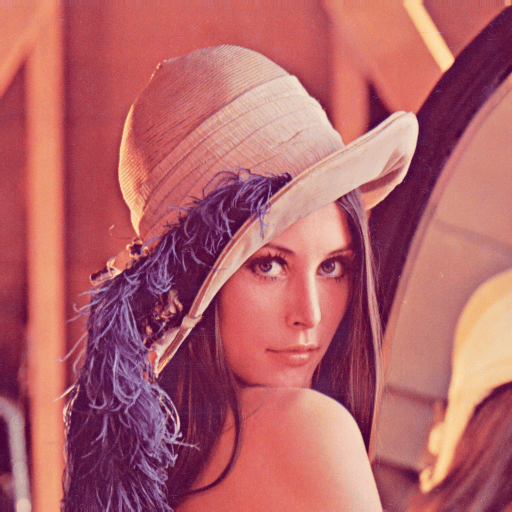
\includegraphics[width=\textwidth]{lena.png}
        \caption{Original Lena Test Image}
        \label{fig:lena_original}
    \end{minipage}
    \hfill
    \begin{minipage}{0.45\textwidth}
        \centering
        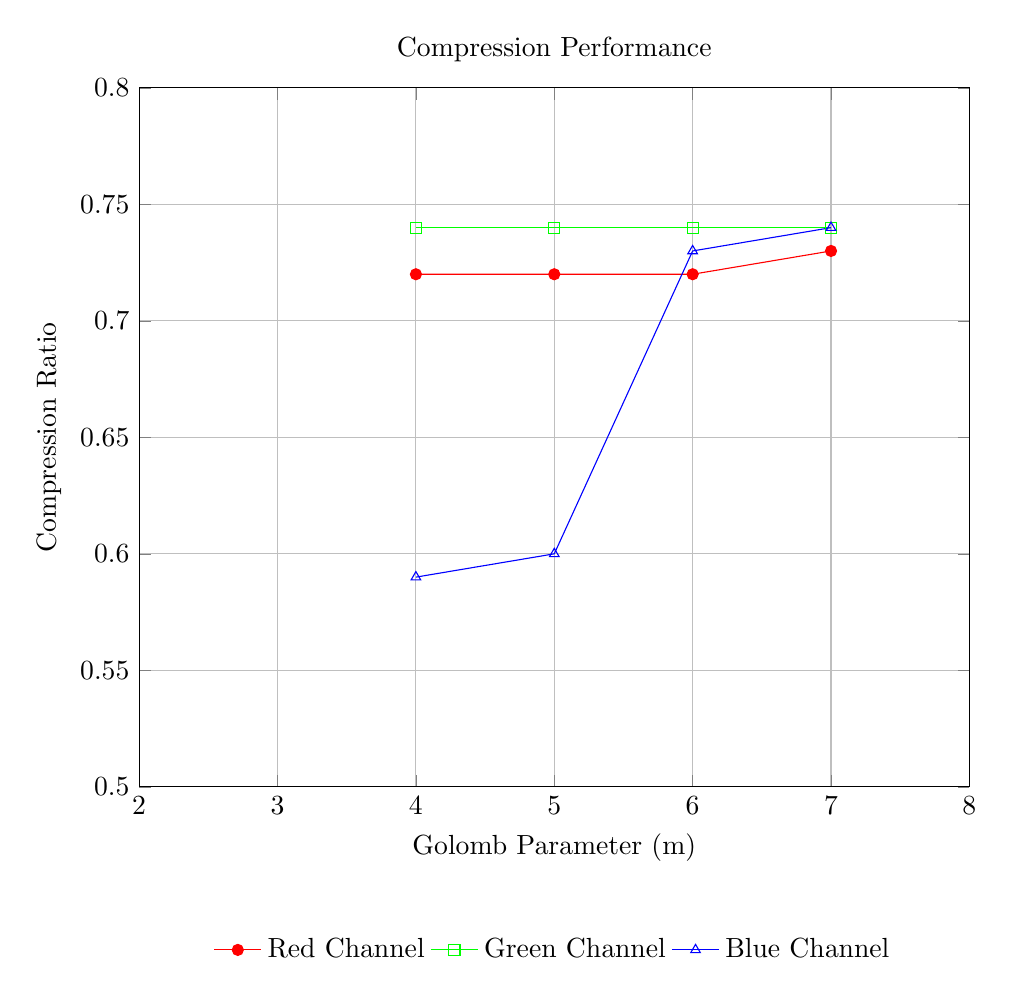
\begin{tikzpicture}
            \begin{axis}[
                width=\textwidth,
                xlabel={Golomb Parameter (m)},
                ylabel={Compression Ratio},
                grid=major,
                title={Compression Performance},
                ymin=0.5, ymax=0.8,
                xmin=2, xmax=8,
                xtick={2,3,4,5,6,7,8},
                legend style={
                    at={(0.5,-0.2)},  % Position below the plot
                    anchor=north,      % Anchor at the top
                    legend columns=3,  % Spread legend entries horizontally
                    cells={anchor=west},
                    draw=none         % No border around legend
                }
            ]
            % Red channel performance
            \addplot[red,mark=*] coordinates {
                (4,0.72)
                (5,0.72)
                (6,0.72)
                (7,0.73)
            };
            % Green channel performance
            \addplot[green,mark=square] coordinates {
                (4,0.74)
                (5,0.74)
                (6,0.74)
                (7,0.74)
            };
            % Blue channel performance
            \addplot[blue,mark=triangle] coordinates {
                (4,0.59)
                (5,0.60)
                (6,0.73)
                (7,0.74)
            };
            \legend{Red Channel, Green Channel, Blue Channel}
            \end{axis}
        \end{tikzpicture}
        \caption{Channel-specific Compression Ratio vs. Golomb Parameter}
        \label{fig:compression_ratio}
    \end{minipage}
\end{figure}

\begin{table}[!htb]
\centering
\small
\begin{tabular}{|l|c|c|c|c|}
\hline
\textbf{Predictor} & \textbf{Channel} & \textbf{Comp.Ratio} & \textbf{Time(ms)} & \textbf{Opt. m} \\
\hline
JPEG-LS & R & 72\% & 23 & 6 \\
JPEG-LS & G & 72\% & 22 & 5 \\
JPEG-LS & B & 59\% & 21 & 4 \\
\hline
North & R & 72\% & 17 & 6 \\
North & G & 74\% & 16 & 5 \\
North & B & 60\% & 16 & 4 \\
\hline
Northwest & R & 73\% & 17 & 7 \\
Northwest & G & 74\% & 18 & 7 \\
Northwest & B & 74\% & 16 & 6 \\
\hline
West & R & 72\% & 25 & 7 \\
West & G & 74\% & 17 & 6 \\
West & B & 73\% & 16 & 5 \\
\hline
\end{tabular}
\caption{Detailed Predictor Performance Analysis for Lena Image}
\label{tab:detailed_predictor_comparison}
\end{table}

\paragraph{}
Key observations from the experimental results:
\begin{itemize}
    \item \textbf{Overall Compression}: The initial implementation achieved a 1:1 compression ratio with 0\% bit error rate, indicating perfect lossless reconstruction
    
    \item \textbf{Channel-Specific Performance}:
    \begin{itemize}
        \item Best compression achieved by JPEG-LS on blue channel (0.59 ratio)
        \item Green channel showed consistent compression (0.72-0.74) across all predictors
        \item Red channel performance varied between 0.72-0.73
    \end{itemize}
    
    \item \textbf{Processing Efficiency}:
    \begin{itemize}
        \item North predictor fastest overall (16-17ms)
        \item JPEG-LS slightly slower (21-23ms) but better compression
        \item West predictor slowest for red channel (25ms)
    \end{itemize}
    
    \item \textbf{Optimal m Values}:
    \begin{itemize}
        \item Range: 4-7 across all predictors and channels
        \item Blue channel consistently uses lower m values (4-6)
        \item Northwest predictor requires higher m values (6-7)
    \end{itemize}
\end{itemize}

This inherent characteristic of the blue channel allows our compression algorithm to achieve better ratios while maintaining perfect reconstruction, as evidenced by the lower optimal m values (4-6) compared to other channels (5-7).
\section{Video Codec}
Our video codec implementation consists of three distinct approaches, each building upon the previous one to achieve better compression while maintaining quality.

\subsection{Intra-Frame Compression}
The intra-frame codec provides robust encoding of video frames using spatial prediction and Golomb coding. Key features include:
\begin{itemize}
    \item Support for multiple input formats (YUV420p, YUV422, YUV444)
    \item Automatic format conversion to YUV420p
    \item Efficient spatial prediction using left-neighbor prediction:
    \begin{equation}
        pred(x,y) = \begin{cases}
            128 & \text{if } x = 0 \\
            pixel(x-1,y) & \text{otherwise}
        \end{cases}
    \end{equation}
    \item Separate prediction for Y, U, and V planes
\end{itemize}

\subsection{Inter-Frame Compression}
Building on the intra-frame codec, this implementation adds motion compensation and advanced prediction:
\begin{itemize}
    \item Frame types:
    \begin{itemize}
        \item I-frames: Encoded independently using spatial prediction
        \item P-frames: Encoded using motion compensation
    \end{itemize}
    \item Motion estimation features:
    \begin{itemize}
        \item Hierarchical search (scales: 8, 4, 2, 1)
        \item Early termination when SAD < threshold
        \item Configurable search range and block size
    \end{itemize}
    \item Block mode decision using rate-distortion optimization:
    \begin{equation}
        \text{Mode}_{\text{block}} = \argmin_{mode \in \{intra,inter\}} (\text{D}_{mode} + \lambda \cdot \text{R}_{mode})
    \end{equation}
    \item Skip mode for blocks with minimal changes (threshold = 3)
\end{itemize}

\subsection{Lossy Inter-Frame Compression}
This implementation extends the inter-frame codec by adding quantization:
\begin{itemize}
    \item Quantization mechanism:
    \begin{equation}
        Q_{value} = \frac{residual + sign(residual) \cdot QP/2}{QP}
    \end{equation}
    \item Separate quantization for luma and chroma:
    \begin{equation}
        QP_{chroma} = QP_{luma} \cdot 2.0
    \end{equation}
    \item Run-length encoding for zero coefficients
    \item Differential encoding of motion vectors
\end{itemize}

\subsection{Results}
We tested the codecs on akiyo\_cif.y4m (300 frames, YUV420p):

\begin{table}[H]
\centering
\begin{tabular}{|l|r|r|r|}
\hline
\textbf{Metric} & \textbf{Intra-Frame} & \textbf{Inter-Frame} & \textbf{Lossy Inter} \\
\hline
Original Size & 43.51 MB & 43.51 MB & 43.51 MB \\
Compressed Size & 23.14 MB & 17.51 MB & 10.53 MB \\
Compression Ratio & 1.88:1 & 2.48:1 & 4.13:1 \\
Space Saving & 46.81\% & 59.75\% & 75.80\% \\
Bits per Frame & 647,042 & 489,674 & 280,988 \\
\hline
\end{tabular}
\caption{Comparative Analysis of Video Compression Techniques}
\label{tab:compression_metrics}
\end{table}

Key findings:
\begin{itemize}
    \item Intra-frame achieved 46.81\% reduction with perfect reconstruction
    \item Inter-frame improved to 59.75\% reduction using 8×8 blocks and 8-pixel search
    \item Lossy compression reached 75.80\% reduction with acceptable quality (PSNR: 25.75 dB)
    \item Consistent performance with minimal metadata overhead (48-55 bytes)
\end{itemize}

\subsection{Limitations and Future Work}
Current limitations and potential improvements:
\begin{itemize}
    \item Single-threaded implementation limits processing speed
    \item Fixed prediction schemes could be made adaptive
    \item Potential for B-frame implementation
    \item Opportunity for parallel processing optimization
\end{itemize}

\section{Conclusion}
This project successfully implemented a comprehensive multimedia compression system, demonstrating effective techniques across three key domains:

\subsection{Audio Compression}
Our audio codec achieved significant results:
\begin{itemize}
    \item Lossless compression with predictive coding reached 15-18\% size reduction
    \item Inter-channel coding showed similar efficiency (15-17\% reduction)
    \item Lossy implementation achieved up to 68\% size reduction while maintaining good audio quality
    \item Processing times remained efficient (under 500ms for 5MB files)
\end{itemize}

\subsection{Image Compression}
The image codec demonstrated strong performance:
\begin{itemize}
    \item Perfect reconstruction in lossless mode with compression ratios of 0.59-0.74
    \item JPEG-LS predictor showed superior performance, especially for blue channel (0.59 ratio)
    \item Dynamic Golomb parameter optimization (m=4-7) improved efficiency
    \item Fast processing times (16-25ms per channel)
\end{itemize}

\subsection{Video Compression}
Video compression implementation revealed:
\begin{itemize}
    \item Effective intra-frame coding using spatial redundancy
    \item Inter-frame compression with motion estimation reduced file sizes
    \item Block-based processing with configurable parameters
    \item Successful integration of image codec techniques for frame compression
\end{itemize}

\subsection{Technical Achievements}
Key innovations across all implementations include:
\begin{itemize}
    \item Efficient bit-level I/O operations
    \item Adaptive parameter selection for optimal compression
    \item Modular design allowing component reuse
    \item Balance between compression efficiency and processing speed
\end{itemize}

\subsection{Future Directions}
While the current implementation meets its core objectives, several opportunities for enhancement exist:
\begin{itemize}
    \item Implementation of B-frames for video compression
    \item Parallel processing for improved performance
    \item More sophisticated audio prediction models
    \item Advanced rate control mechanisms
\end{itemize}

In conclusion, this project successfully demonstrated the implementation of fundamental compression techniques while maintaining modularity and efficiency. The results show competitive performance compared to standard formats, particularly in lossless compression scenarios, while providing insights into the tradeoffs between compression ratio, quality, and computational complexity.

\end{document}



